%---------------------------------------------------------------------------%
%-                                                                         -%
%-                           LaTeX Template                                -%
%-                                                                         -%
%---------------------------------------------------------------------------%
%- Copyright (C) Huangrui Mo <huangrui.mo@gmail.com> 
%- This is free software: you can redistribute it and/or modify it
%- under the terms of the GNU General Public License as published by
%- the Free Software Foundation, either version 3 of the License, or
%- (at your option) any later version.
%---------------------------------------------------------------------------%
%->> Document class declaration
%---------------------------------------------------------------------------%
\documentclass[singlesided]{Style/ucasthesis}%
%- Multiple optional arguments:
%- [<singlesided|doublesided|printcopy>]% set one or two sided eprint or print
%- [draftversion]% show draft version information
%- [fontset=<fandol|...>]% specify font set to replace automatic detection
%- [scheme=plain]% thesis writing of international students
%- [standard options for ctex book class: draft|paper size|font size|...]%
%---------------------------------------------------------------------------%
%->> Document settings
%---------------------------------------------------------------------------%
\usepackage[super,myhdr,tikz,list,math]{Style/artratex}% document settings 文档设定
%- usage: \usepackage[option1,option2,...,optionN]{artratex}
%- Multiple optional arguments:
%- [bibtex|biber]% set bibliography processor and package   %参考文献
%- [<numbers|super|authoryear|alpha>]% set citation and reference style  %设置参考文献格式
%- <numbers>: textual: Jones [1]; parenthetical: [1]
%- <super>: textual: Jones superscript [1]; parenthetical: superscript [1]
%- <authoryear>: textual: Jones (1995); parenthetical: (Jones, 1995)
%- <alpha>: textual: not available; parenthetical: [Jon95]
%- [geometry]% reconfigure page layout via geometry package   % 设置页面各部分尺寸。常用
%- [lscape]% provide landscape layout environment             %提供
%- [myhdr]% enable header and footer via fancyhdr package     %
%- [color]% provide color support via xcolor package
%- [background]% enable page background
%- [tikz]% provide complex diagrams via tikz package     %配合pgf宏包创建复杂图表x
%- [table]% provide complex tables via ctable package    %表格
%- [list]% provide enhanced list environments for algorithm and coding  %用于算法或编码的
%- [math]% enable some extra math packages    %提供额外的数学包
\usepackage{Style/artracom}% user defined commands
\usepackage{graphicx}
\usepackage{amsmath}

%%%%%%%%%%%%%%%%%%%%%%%%%%%%%%%%%%%%%%%%%%%%%%%%%%%%%%%%%%%%%%%%%%%%%%%%%%%%%%%%%%%%%%%%%%%%%%%%%%%%
\usepackage{amsfonts,amssymb,bm}
\usepackage{mathrsfs}
%
%\newtheoremstyle{theoremwithoutdot}% 类型名
%{}%                   Space above, empty = `usual value'
%{}%                   Space below
%{\kaishu}%                   Body font
%{}%         Indent amount (empty = no indent, \parindent = para indent)
%{\heiti}%          Thm head font
%{}%                   Punctuation after thm head
%{1em}%                Space after thm head
%{\thmname{#1}\thmnumber{~#2}\thmnote{~(#3)}}%                   Thm head spec
%
%\newtheoremstyle{solutionstyle}% 类型名
%{}%                   Space above, empty = `usual value'
%{}%                   Space below
%{}%                   Body font
%{}%         Indent amount (empty = no indent, \parindent = para indent)
%{\heiti}%          Thm head font
%{}%                   Punctuation after thm head
%{1em}%                Space after thm head
%{\thmname{#1}\thmnumber{~#2}\thmnote{~(#3)}}%                   Thm head spec
%\theoremstyle{theoremwithoutdot}
\newtheorem{defi}{定义}[section]
\newtheorem{theorem}{定理}[section]
\newtheorem{lemma}[theorem]{引理}
\newtheorem{prop}[theorem]{命题}
\newtheorem{coro}{推论}[theorem]
\newtheorem{remark}{注}
%\newtheorem{atten}{注意:}
\newtheorem{example}{例}[chapter]
\newtheorem{question}{题}[section]
\newtheorem{property}[theorem]{性质}
\renewcommand{\thequestion}{\arabic{chapter}.\arabic{section}.\arabic{question}}
%\theoremstyle{solutionstyle}
%\newtheorem*{solution}{解}

%%%%%%%%%%%%%%%%%%%%%%%%%%%%%%%%%%%%%%%%%%%%%%%%%%%%%%%%%%%%%%%%%%%%%%%%%%%%%%%%%%%%%%%%%%%%%%%%%%%

%---------------------------------------------------------------------------%
%->> Document inclusion
%---------------------------------------------------------------------------%
%\includeonly{Tex/Chap_1,...,Tex/Chap_N}% selected files compilation
%---------------------------------------------------------------------------%
%->> Document content
%---------------------------------------------------------------------------%
\begin{document}
%-
%-> Frontmatter: title page, abstract, content list, symbol list, preface
%-
%\frontmatter% initialize the environment
%%---------------------------------------------------------------------------%
%->> 封面信息及生成
%---------------------------------------------------------------------------%
%-
%-> 中文封面信息
%-
\confidential{}% 密级:只有涉密论文才填写
\schoollogo{scale=0.095}{ucas_logo}% 校徽
\title{}% 论文中文题目
\author{}% 论文作者
\advisor{}% 指导教师:姓名 专业技术职务 工作单位
\advisorsec{}% 指导老师附加信息 或 第二指导老师信息
\degree{}% 学位:学士、硕士、博士
\degreetype{}% 学位类别:理学、工学、工程、医学等
\major{}% 二级学科专业名称
\institute{}% 院系名称
\chinesedate{}% 毕业日期:夏季为6月、冬季为12月



%-> 中文封面信息
%-
%\confidential{}% 密级:只有涉密论文才填写
%\schoollogo{scale=0.095}{ucas_logo}% 校徽
%\title{中国科学院大学学位论文\LaTeX{}模板 {$~^{\pi}\pi^{\pi}$}}% 论文中文题目
%\author{莫晃锐}% 论文作者
%\advisor{刘青泉~研究员~中国科学院力学研究所}% 指导教师:姓名 专业技术职务 工作单位
%\advisorsec{}% 指导老师附加信息 或 第二指导老师信息
%\degree{硕士}% 学位:学士、硕士、博士
%\degreetype{理学}% 学位类别:理学、工学、工程、医学等
%\major{流体力学}% 二级学科专业名称
%\institute{中国科学院力学研究所}% 院系名称
%\chinesedate{2014~年~6~月}% 毕业日期:夏季为6月、冬季为12月
%-
%-> 英文封面信息
%-
\englishtitle{\LaTeX{} Thesis Template\\ of \\ The University of Chinese Academy of Sciences {$~^{\pi}\pi^{\pi}$}}% 论文英文题目
\englishauthor{Mo Huangrui}% 论文作者
\englishadvisor{Supervisor: Professor Liu Qingquan}% 指导教师
\englishdegree{Master}% 学位:Bachelor, Master, Doctor。封面格式将根据英文学位名称自动切换,请确保拼写准确无误
\englishdegreetype{Natural Science}% 学位类别:Philosophy, Natural Science, Engineering, Economics, Agriculture 等
\englishthesistype{thesis}% 论文类型: thesis, dissertation
\englishmajor{Fluid Mechanics}% 二级学科专业名称
\englishinstitute{Institute of Mechanics, Chinese Academy of Sciences}% 院系名称
\englishdate{June, 2014}% 毕业日期:夏季为June、冬季为December
%-
%-> 生成封面
%-
\maketitle% 生成中文封面
%\makeenglishtitle% 生成英文封面
%-
%-> 作者声明
%-
%\makedeclaration% 生成声明页
%-
%-> 中文摘要
%-
%\chapter*{摘\quad 要}\chaptermark{摘\quad 要}% 摘要标题
%\setcounter{page}{1}% 开始页码
%\pagenumbering{Roman}% 页码符号
%
%本文是中国科学院大学学位论文模板ucasthesis的使用说明文档。主要内容为介绍\LaTeX{}文档类ucasthesis的用法,以及如何使用\LaTeX{}快速高效地撰写学位论文。
%
%\keywords{中国科学院大学,学位论文,\LaTeX{}模板}% 中文关键词
%%-
%%-> 英文摘要
%%-
%\chapter*{Abstract}\chaptermark{Abstract}% 摘要标题
%
%This paper is a help documentation for the \LaTeX{} class ucasthesis, which is  a thesis template for the University of Chinese Academy of Sciences. The main content is about how to use the ucasthesis, as well as how to write thesis efficiently by using \LaTeX{}.
%
%\englishkeywords{University of Chinese Academy of Sciences (UCAS), Thesis, \LaTeX{} Template}% 英文关键词
%%---------------------------------------------------------------------------%
% title page, abstract, dedication
{% content list region
\linespread{1.2}% local line space
%\intotoc{\contentsname}% add link to contents table and bookmark
\tableofcontents% contents catalog
%\intotoc{\listfigurename}% add link to contents table and bookmark
%\listoffigures% figures catalog
%\intotoc{\listtablename}% add link to contents table and bookmark
%\listoftables% tables catalog
}
%\chapter*{符号列表}
\chaptermark{符号列表}

\section*{字符}
\nomenclatureitem[\textbf{Unit}]{\textbf{Symbol}}{\textbf{Description}}
\nomenclatureitem[$\Unit{m^{2} \cdot s^{-2} \cdot K^{-1}}$]{$R$}{the gas constant}
\nomenclatureitem[$\Unit{m^{2} \cdot s^{-2} \cdot K^{-1}}$]{$C_v$}{specific heat capacity at constant volume}
\nomenclatureitem[$\Unit{m^{2} \cdot s^{-2} \cdot K^{-1}}$]{$C_p$}{specific heat capacity at constant pressure}
\nomenclatureitem[$\Unit{m^{2} \cdot s^{-2}}$]{$E$}{specific total energy}
\nomenclatureitem[$\Unit{m^{2} \cdot s^{-2}}$]{$e$}{specific internal energy}
\nomenclatureitem[$\Unit{m^{2} \cdot s^{-2}}$]{$h_T$}{specific total enthalpy}
\nomenclatureitem[$\Unit{m^{2} \cdot s^{-2}}$]{$h$}{specific enthalpy}
\nomenclatureitem[$\Unit{kg \cdot m \cdot s^{-3} \cdot K^{-1}}$]{$k$}{thermal conductivity}
\nomenclatureitem[$\Unit{kg \cdot m^{-1} \cdot s^{-2}}$]{$S_{ij}$}{deviatoric stress tensor}
\nomenclatureitem[$\Unit{kg \cdot m^{-1} \cdot s^{-2}}$]{$\tau_{ij}$}{viscous stress tensor}
\nomenclatureitem[$\Unit{1}$]{$\delta_{ij}$}{Kronecker tensor}
\nomenclatureitem[$\Unit{1}$]{$I_{ij}$}{identity tensor}

\section*{算子}
\nomenclatureitem{\textbf{Symbol}}{\textbf{Description}}
\nomenclatureitem{$\Delta$}{difference}
\nomenclatureitem{$\nabla$}{gradient operator}
\nomenclatureitem{$\delta^{\pm}$}{upwind-biased interpolation scheme}

\section*{缩写}
\nomenclatureitem{CFD}{Computational Fluid Dynamics}
\nomenclatureitem{CFL}{Courant-Friedrichs-Lewy}
\nomenclatureitem{EOS}{Equation of State}
\nomenclatureitem{JWL}{Jones-Wilkins-Lee}
\nomenclatureitem{WENO}{Weighted Essentially Non-oscillatory}
\nomenclatureitem{ZND}{Zel'dovich-von Neumann-Doering}

% list of symbols, preface content
%-
%-> Mainmatter
%-
\mainmatter% initialize the environment
%---------------------------------------------------------------------------%
%->> Main content
%---------------------------------------------------------------------------%
\chapter{绪论}\label{chap:introduction}

\section{概述}
\subsection{稀疏建模:时代的需要}
获取信息,从而认识大千世界,是人类文明发展的主旋律。在目前智能时代,信息时代的发展过程中,各种传感器技术快速发展,数量不断增长,硬件成本减低,数据量呈现爆炸式增长。数据洪流给传统的数据存储,传输处理方法带来了巨大的压力。海量数据促使新的方法:从数据中学习,形成信号表达,信号获取与复原的新概念和新方法。

自然界的大多数信号具有一定的结构性,结构性信号的自由度要远低于信号本身的维度。海量数据的典型特征就是信息冗余,其携带的信息量非常有限。可以用稀疏性来描述这个特性。

信息表达的研究表明,几乎在所有的情况下,数据中携带的信息量是稀疏的。
可以说稀疏性是海量数据的本质特性之一,正是这个特性,为海量数据的的表达和处理提供了便利,为更有效的数据解译提供了可能。

信号表达的基本任务是描述信号组成的基本要素,揭示信号组织和生成的方式。离散余弦变换和小波变换等经典信号仅描述了信号的基本要素和简单线性组织方法,不能揭示信号深层次的组织和生成方式。

在统计分析和机器学习的驱动下,从数据中学习信号特征的表达方法开始出现,信号表达进入基于学习的表达方法中。

\subsection{稀疏建模的哲学基础:剃刀原则}
稀疏建模,是节省性原则在现代统计学,机器学习和信号处理领域的特殊体现。在这些领域,一个基础性的问题就是,由于观测成本或其他限制,需要从数量相对较少的观测中对未观测高维信号进行精确复原。

一般的,高维小样本推断问题是欠定的,且在计算上是难以处理的,除非该问题具有某一特定的结构,例如稀疏性。

事实上,当仅有少量变量为真正重要的变量时,真实解可以很好的由稀疏向量来近似,将剩余变量设置为0或者接近0。换言之,少量最相关的变量(起因,预测因子等),通常对于解释感兴趣的现象来说是充分的。

更一般的,即使原始问题没有产生稀疏解,我们可以找到一个映射(或字典),将其映射到新的坐标系统,从而实现稀疏表示。因此稀疏机构看上去是很多自然信号固有的性质,没有该结构,认知并适应这个世界是相当具有挑战性的问题。

\section{问题的提出}
如何从有限的观测中推断出未被观测到的高维“世界状态”,这个问题常常出现在广泛的实际应用中。



\begin{enumerate}
	\item 寻找基因中引发某种疾病的子集;
	\item 定位与某一心理状态存在关联的大脑区域	
	\item 诊断大规模分布式计算机系统中的性能瓶颈
	\item 使用压缩观测值重构高质量的图像
\end{enumerate}

更一般的例子是,从任意一类信号的含噪编码中对信号解码,以及在高维但小样本的统计情况下估计模型参数。

图xx描述的就是这种基本推断难问题,其中$x=(x_1,x_2,\cdots,x_n)$代表一个未被观测的n维的世界状态,$y=(y_1,y_2,\cdots,y_m)$代表它的m个观测结果。观测结果的输出向量y可以看成是输入向量x的一个含噪函数(编码)。
\begin{figure}[th]
	\centering
	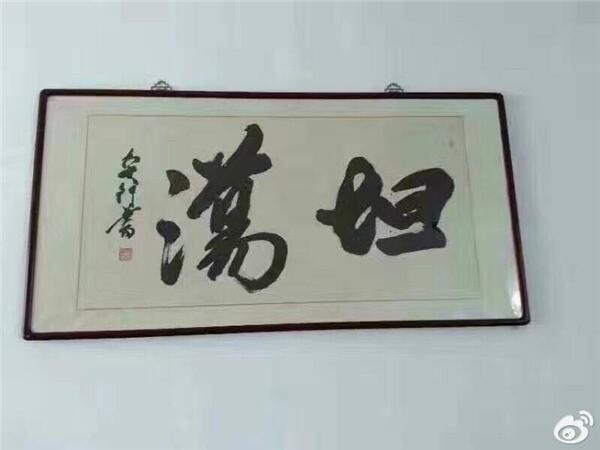
\includegraphics[width=0.5\linewidth]{Img/Chap_Intro/fig1_1}
	\caption[hello]{hellohello}
	\label{fig:test}
\end{figure}
一种常用的推断(解码)方法是,给定观测结果y,找到某种损失函数$L(x;y)$,使之最小化得到x。例如常见的极大似然法,就是旨在找到一个使得观测结果的似然$P(y|x)$最大化的参数向量x。

然而在许多实际问题中,未被观测到的变量在数量上远远多于观测值,因为对真实世界的观测成本很高,且受到具体问题的限制。通常未知变量的总数可能达到数千个或上百万个,而观测结果或者样本数量总数通常只有几百个。因此上述似然表达式将变为欠定情况。

同时,为了限定可能的解空间,必须引入额外的,反映了特定领域性质或假设的正则化约束。从贝叶斯概率的假设来说,正则化可以看做是对未知参数四家了先验$P(x)$,然后最大化后验概率$P(x|y)=P(y|x)P(x)/P(y)$。

或许,关于问题结构做的最简单、最常见的假设之一是解为稀疏的。换言之,通常假定在特定情况下,只有一个相对较小的变量子集是真正重要的。例如:
\begin{itemize}
	\item 一个系统只出现少量的并发故障;
	\item 只需要少数非零傅里叶系数就能满足对不同信号类型的准确表示;
	\item 只有一小部分预测变量(如基因)与响应变量(疾病或特征)最相关;
	\item 学习某一精确预测模型也只需要一小部分预测变量。
\end{itemize}
在这些例子中,我们寻求的解可以看成是一个仅有少量非零坐标的稀疏高维向量。这一假设与哲学中的节省性原则一致,而这一原则通常被称为奥卡姆剃刀原则,由中世纪著名哲学家奥卡姆威廉提出。之前可追溯到亚里士多德和托勒密,之后也出现了许多关于节省性原则的阐述,其中包括牛顿的著名表述:“寻求自然事物的本因,只需找到真实而又足以解释其现象即可,无需更多。”


\subsection{欠定线性系统}

线性代数的可用于对对线性方程组求,对该问题进行彻底考查。而线性方程组求解是很多工程应用和解决方案的核心问题。令人惊讶的是,在这个问题中,却有一个不得不用线性系统的稀疏解来解决的初级问题,该问题最近才被深入的探索和研究。

{\heiti 
我们会发现这个解有很令人惊讶的答案,它促进了很多的实际发展。在这一章中我们应该集中精力认真的定义这个问题,为在以后的章节中的问题答案做好准备。}


设有一个矩阵$A\in R^{n\times m}(n<m)$,定义一个由线性方程组$Ax=b$描述的\emph{欠定系统}。该欠定系统中,未知数多于方程式数目。如果向量b不在矩阵A列向量张成的空间中,则这个系统无解。否则,方程有无穷多个解。为避免这种异常情况发生,本书中假设A为一个满秩矩阵,既其列向量张成整个$R^n$空间。

这种欠定线性系统求解的问题,我们在工程中常常碰到。例如:
{\heiti
图像处理中的上采样问题,一副未知图像x经过模糊和下采样,将得到一副低质量小图像b。矩阵A代表了这种退化操作。我们的目标就是从观测b中重构出原始图像x。
}
显然,有无数中图像x能用来解读降质图像b,但其中总有一些看起来更好一些,问题是我们怎么去寻找最好,最合适和最准确的x呢?


\subsection{正则化解}
在上面的例子中,我们总希望得到唯一解,但我们面临的最大障碍是,其可能存在无穷解。为了将选择范围缩小为一个满意解,显然需要增加条件。

一个常用的增加条件的方法,就是正则化(regularization),即引入一个对x的候选解进行合理性评价的函数$J(x)$,并期望其值越小越好,对常规的优化问题$(P_J)$可做如下定义:
\begin{equation}
	(P_J):\quad  \min_{x}J(x)\quad s.t.\quad b=Ax
\end{equation}
\par 现在可用$J(x)$来约束可能解的类型。如在图像上采样用,一般用$J(x)$表征$x$的光滑度,或分段光滑度。

但最常见的J(x)函数是欧式范数的平方$\Vert{x}\Vert^2_2$。事实上这种选择带来的$(P_2)$问题存在唯一解$\hat{x}$。可利用拉格朗日法对其求解。

定义拉格朗日公式:
\begin{equation}%\label{key}
L(x)= \Vert x \Vert_2^2 + \lambda^{T}(Ax-b)
\end{equation}

这里$\lambda$为约束集合所对应的拉格朗日乘子。将上式两边对$ \lambda $求导可得:
\begin{equation}\label{key}
\frac{\partial L(x)}{\partial\lambda}= 2 x  +A^{T}\lambda 
\end{equation}

令其等于0,由此得到解如下:
\begin{equation}\label{key}
\hat{x}_{opt} = -\frac{1}{2} A^T \lambda
\end{equation}

将这个 解带入约束条件$ Ax=b $,可得:
\begin{equation}\label{key}
A\hat{x}_{opt} = -\frac{1}{2} A A^T \lambda = b  \Longrightarrow
 \lambda = -2(AA^T)^{-1}b 
\end{equation}

再将该结果带入式1-4,就可以得到常见的闭合形式的伪逆解:
\begin{equation}\label{key}
\hat{x}_{opt} = -\frac{1}{2} A^T \lambda = A^{T}(AA^T)^{-1}b  = A^{+}b
\end{equation}


欧式范数被广泛的应用于各个工程的领域,主要在于其比较简单,可以给出上述闭合形式的唯一解。在信号和图像处理中,这种正则化处理被广泛应用于各种逆问题求解,信号表示等领域。但其并不是真正的最佳选择。





































\section{稀疏表示的研究概况}

过去几年,稀疏性相关研究已经远远超出了原来信号复原理论描述的范畴,涵盖了:
\begin{enumerate}
	\item 稀疏非线性回归,如广义线性模型
	\item 稀疏概率网络,如马尔科夫网络和贝叶斯网络
	\item 稀疏矩阵分解,如字典学习
	\item 稀疏主成分分析,
	\item 稀疏非负矩阵分解
	\item 稀疏贝叶斯学习
\end{enumerate}


此外,由于稀疏建模领域存在大量的新进展,一些重要的问题例如低秩矩阵完备,在很多应用中出现,包括协同过滤、度量学习、多任务学习等,由于秩最小化问题类似于$ \ell_0 $范数最小化,非常难以处理,通常可以通过迹范数(或称为核范数)来利用凸松弛,其中迹范数即为奇异值向量的$ \ell_1 $范数。


                  %绪论

\part{小波变换:\\理论及其在图像处理中的应用}
%%%hello           %小波分析理论
%%%hello        %二维小波变换     
%%%hello         %小波变换应用
\part{稀疏表示:\\理论和数值基础}
\chapter{稀疏复原:问题描述}\label{chap:srt01:problem}

本章的主要内容为稀疏信号复原中的优化问题。

从一个简单的不含噪线性观测情况开始,将之扩展为更为实际的含噪复原问题。问题的最终目的是寻找最稀疏解,也就是包含最少非零值的解,也称为$\ell_0$范数解,但由于其非凸组合本质,在计算上非常困难(确切地说是NP难问题),因此其求解必须借助近似方法。

稀疏复原中通常使用两种主要的近似方法,第一种是通过诸如贪婪搜索这样的近似方法来解决原始的NP难问题。第二种方法则是利用易于求解的凸松弛来代替棘手的原NP难问题。换言之,前者以近似方法解决精确问题,后者以精确方式解决近似问题。

考虑边界为$ \ell_0 $范数的$ \ell_p $范数族,并重点研究$ \ell_1 $范数,因为$ \ell_1 $范数是整个$ \ell_p $范数族中唯一能产生稀疏性并同时保持凸性的范数。

最后,从贝叶斯估计角度讨论稀疏信号复原和稀疏统计学习,引出最大后验概率参数估计(MAP)。与MAP方法相联系的是正则化优化,其中负对数似然和参数的先验分别对应损失函数和正则函数。

\section{不含噪稀疏复原}

继续使用之前的符号表示:$\mathit{x}=(x_1,x_2,\cdots,x_n)^T\in \mathbb{R}^N$为未观测的稀疏信号,$ y=(y_1,y_2,\cdots,y_m)^T\in \mathbb{R}^m $为观测值或观测向量,而$ A={a_{ij}}\in \mathbb{R}^{m\times n} $为设计矩阵。

从根据一组线性观测值复原无噪声信号这样最简单的问题开始,即求解线性方程组中的$ x $,
\begin{equation}\label{key}
Ax=y
\end{equation}
这里通常假设A是一个满秩矩阵,这样,对于任何$ y\in \mathbb{R}^m $,上述方程组有解。但需要注意的是,当未知变量的数量,即信号的维度,超过了观测值的数量,即$ m\leq n $时,上述方程组是欠定的,存在无数多个解。

为了复原信号$ x $,需要进一步对问题进行约束,或称为正则化。一般通过引入一个目标函数(或正则函数)$ R(x) $,以对信号额外的性质进行编码来实现,该目标函数或正则函数在取得期望解时具有较低值。因此,信号复原问题可以表述为以下约束优化问题:
\begin{equation}\label{key}
\min_{x\in \mathbb{R}^n}\: R(x)\quad s.t.\quad y=Ax
\end{equation}
例如,当希望得到的解具有稀疏性时,$ R(x) $就可以定义为非零元素的数量,或称为x的势,也称为$ \ell_0 $范数,表示为$ \Vert x \Vert_0 $。当腰注意,$ \ell_0 $范数并非严格意义上的范数,这一点会简要讨论。

一般的,特定$q$值的$ \ell_q $范数(表示为$ \Vert x \Vert_q $),经常用作正则函数,但更常见的是使用$ \ell_q $范数的$q$次幂$ \Vert x \Vert_q^q $作为正则函数。

现在详细研究$ \ell_q $范数的及其性质。当$ q\geq 1 $时,$ \ell_q $范数定义为:
\begin{equation}\label{key}
\Vert x \Vert_q = \left(\sum_{i=1}^{n}|x_i|^q\right)^{\frac{1}{q}}
\end{equation}


\begin{enumerate}
	\item 当$ q=2 $时,即为$ \ell_2 $范数,也称为欧几里得范数,是最常用的$ \ell_q $范数。
	\begin{equation}\label{key}
		\Vert x \Vert_2 = \sqrt{\sum_{i=1}^{n}|x_i|^2}
	\end{equation}
	\item 当$ q=1 $时,即为$ \ell_1 $范数。
	\begin{equation}\label{key}
		\Vert x \Vert_1 = \sum_{i=1}^{n}|x_i|
	\end{equation}
\end{enumerate}

现在我们回到向量的势及其与$ \ell_q $范数的关系。函数$ \Vert x \Vert_0 $被称为$ x $的$ \ell_0 $范数,定义为$ \Vert x \Vert_q^q $的极限,即当$ q\rightarrow 0 $时$ \ell_q $范数的第$ q $次幂:
\begin{equation}\label{key}
\Vert x \Vert_0 = \lim_{q\rightarrow 0}\Vert x \Vert_q^q = \lim_{q\rightarrow 0} \sum_{i=1}^{p}| x_i |^q = \sum_{i=1}^{p}\lim_{q\rightarrow 0} | x_i |^q
\end{equation}

而对于每一个$ x_i $,当$ q\rightarrow 0 $时,有$ |x_i\rightarrow I(x_i) $。$ x=0 $时,$ I(x) $值为0,否则为1.
因此可得,$\Vert x \Vert_0=\sum_{i=1}^{p}I(x_i)$,这给出了向量$ x $中非零元素的精确数量,也被称为势。利用势函数,现在可以将从不含噪线性观测值中复原稀疏信号的问题写成如下形式:
\begin{equation}\label{key}
(P_0):\quad  \min_{x} \Vert x \Vert_0 \quad s.t. \quad y =Ax
\end{equation}

上式中定义的$ (P_0) $问题是一个NP难问题,即目前没有算法能够在多项式时间内对其高效的求解。因此有必要借助近似方法。在恰当的条件下,最优或近似最优的解可以通过某近似方法来高效复原。
以下为两种常用的近似方法:
\begin{enumerate}
	\item {\heiti 利用基于启发式的搜索过程},如通过贪婪搜索以探寻问题$ (P_0) $的解空间。
	\begin{enumerate}
		\item 例如,可以从一个零向量开始,逐个增加非零坐标,在每一步中选择能够对目标函数值带来最佳该井的坐标。也叫贪婪坐标下降法。
		\item 一般地,这种启发式搜索方法并不能保证找到全局最优解。
		\item 但这种方法在实践中容易实现,计算效率非常高,并且常常能找到足够优的解。
	\end{enumerate}
    \item {\heiti 松弛方法},这种方法利用易处理的目标函数或约束来代替那些难以处理的目标函数
    \begin{enumerate}
    	\item 例如,凸松弛方法通过凸优化问题来近似非凸优化问题,也就是通过包含凸目标和凸约束的问题来近似非凸优化问题。
    	\item 这种凸优化问题通常是比较容易求解,存在很多优化方法来求解凸问题。
    	\item 显然,松弛的$ (P_0) $问题还必须保证解的稀疏性。
    \end{enumerate}
\end{enumerate}
\subsection{凸性的简单回顾}
几个概念:
\begin{enumerate}
	\item {\heiti 凸组合:} \\
	
	给定两个向量$ x_1\in \mathbb{R}^n $和量$ x_2\in \mathbb{R}^n $,以及一个标量 $ \alpha\in[0,1] $,向量$ x=\alpha x_1+(1-\alpha) x_2 $称为$ x_1 $和$ x_2 $的凸组合。
	\item {\heiti 凸集:}  \\
	
	如果集合$ S $中任何元素组成的凸组合任然属于该集合,那么该集合就称为凸集,即
	\[ \forall x_1,x_2 \in S,\quad\forall\alpha\in [0,1], \mbox{如果} x=\alpha x_1+(1-\alpha) x_2,\mbox{则} x\in S\]
	\item {\heiti 凸函数:} \\
	
	在一个向量空间上,定义于凸集合S上的函数$ f(x):S\rightarrow\mathbb{R} $称为凸函数的条件是
	\[ \forall x_1,x_2 \in S,\;\forall\alpha\in [0,1], \quad f(\alpha x_1+(1-\alpha) x_2)\leq \alpha f(x_1) + (1-\alpha)f(s_2) \]
	\begin{enumerate}
		\item 也就是说,连接凸函数曲线上两个点的线段总处于该函数曲线上方。
		\item 从几何角度来看,另一点解释方式是函数曲线上方的点组成的集合是凸的
		\item 如果上面的不等式是严格的,则该函数被称为严格凸函数
		\item 假设$ x_1 \neq x_2 $,且$ 0<\alpha<1 $,则凸函数的一个重要性质是其任意局部最小值也是全局最小值。而且严格凸函数具有唯一全局最小值。
	\end{enumerate}
\end{enumerate}

凸优化问题是凸函数在可行解的凸集上的最小化,其中可行解由约束来定义。由于凸目标函数的特性,凸问题比一般的优化问题易于求解。凸优化是优化相关文献中的一个传统研究领域,并且在过去若干年中已经有了许多高效的求解方法。

\subsection{问题$P_0$的松弛}
回到原问题$(P_0)$,即具有线性约束的势最小化。显然,约束$ y=Ax $产生了一个凸的可行集。事实上,给定两个满足这一约束的可行解$ x_1,x_2 $,两者的任意凸组合也是可行解。因为:
$$ A(\alpha x_1+(1-\alpha) x_2) = \alpha Ax_1 +(1-\alpha)Ax_2 = \alpha y+ (1-\alpha)y =y$$

因此,为了使问题$ (P_0) $松弛为一个凸问题,只需要用一个凸函数来代替目标函数$\Vert x \Vert_0  $,当然这里主要关注$ \ell_q $范数并将其作为$ \ell_0 $可能的松弛方法。

更精确的说,我们将研究$ \ell_q $范数的$ q $次幂,即函数$ \Vert x\Vert_q^q $,作为一般情况下的正则化函数$ R(x) $。对于一般情况下,当$ q\geq 1 $时,该函数为凸函数,当$ q<1 $时,其为非凸函数。


{\heiti 例如,$ \ell_2 $范数作为使用最广泛的$ \ell_q $范数,将其作为$ \ell_0 $范数的松弛也是自然而然的第一选择,可以得到问题$ (P_2) $}。
\begin{equation}\label{key}
(P_2):\quad  \min_{x} \Vert x \Vert_2^2 \quad s.t. \quad y =Ax
\end{equation}

函数$ \Vert x\Vert_2^2 $是严格凸的,并且具有唯一最小值。此外,问题$ (P_2) $具有解析闭合解。

{\heiti 求解问题$ (P_2) $可利用拉格朗日法。}

定义拉格朗日公式:
\begin{equation*}%\label{key}
\mathcal{L}(x)= \Vert x \Vert_2^2 + \lambda^{T}(y-Ax)
\end{equation*}

这里$\lambda$为一m维向量,其约束集合所对应的拉格朗日乘子。将上式两边对$ \lambda $求导可得::
\begin{equation*}\label{key}
\frac{\partial \mathcal{L}(x)}{\partial\lambda}= 2 x  +A^{T}\lambda 
\end{equation*}

令其等于0,即为上式的最优化条件。可得到唯一最优解如下:
\begin{equation*}\label{chap_srt01_x_l2opt}
x^*= -\frac{1}{2} A^T \lambda
\end{equation*}

因为$ x^* $必须满足约束条件$y= Ax$,将这个解带入约束条件,可得$ \lambda = -2(AA^T)^{-1}y $,即:
\begin{equation*}\label{key}
Ax* = -\frac{1}{2} A A^T \lambda = y  \Longrightarrow
\lambda = -2(AA^T)^{-1}y 
\end{equation*}

再将该结果带入式(\ref{chap_srt01_x_l2opt}),就可以得到常见的闭合形式的解析解:
\begin{equation*}\label{key}
x^* = -\frac{1}{2} A^T \lambda = A^{T}(AA^T)^{-1}b  = A^{+}b
\end{equation*}

当A的列数比行数多时,这个解被称为$ y=Ax $的伪逆解,这里要假定A是满秩的,即所有的行都是线性独立的。然而$\Vert x\Vert_2^2  $目标函数具有一个严重的缺陷,其最优解不是稀疏的,无法再稀疏信号复原中成为一个很好的近似方法。

\subsection{$\ell_q$-正则函数对接的稀疏性的影响}

{\heiti 如果你要要理解为何$ \ell_2 $范数无法得到解的稀疏性,而$ \ell_0 $范数却可以,要理解$ \ell_q $范数的凸性,以及导致稀疏的性质,则需要研究问题$ (P_q) $的几何结构。}
\begin{equation}\label{key}
(P_q):\quad  \min_{x} \Vert x \Vert_q^q \quad s.t. \quad y =Ax
\end{equation}

注意:{\heiti 	使得函数$ f(x) $具有相同值,即$ f(x)=const $的向量集合称为函数$ f(x) $的水平集。}
\begin{enumerate}
	\item 满足$ \Vert x\Vert_q^q \leq r^q $的向量集合称为半径为r的$\ell_q $球,其“表面”(集合边界)即为相应的水平集。
	\item 对于$ q\geq 1 $来说,以水平集为边界的$\ell_q $球是凸的,球上两点之间的直线仍在球内。
	\item 对于$ 0< q< 1 $来说,以水平集为边界的$\ell_q $球是非凸的,球上两点之间的直线并不总在球内。
\end{enumerate}

显然:{\heiti 	从几何视角来看,求解问题$ (P_q) $等价于以原点为中心“吹起”$ \ell_q $球,也就是说从0开始增加$ \ell_q $球半径,直到与超平面$ y=Ax $相交。相交点为最小$ \ell_q $范数向量。同时也是一个可行解,即为$ (P_q) $问题的最优解。}

注意,当$ q\leq 1 $时,$ \ell_q $球在坐标轴上有尖角,这些尖角与稀疏向量相对应,因为尖角的某坐标为0;但是当$ q>1 $时,$ \ell_q $球无此性质。因此,{\heiti 对于$ q\leq 1 $时,$ \ell_q $球可能与超平面$ Ax=y $在尖角处相交,从而产生稀疏解},而对于$ q>1 $,交点在实际中并不能在坐标轴上发生,解并不具有稀疏性。这是一个对$ \ell_q $范数性质直观的论证。

总的来说,我们既想要一个容易优化的函数来近似难于处理的$ \ell_0 $优化问题,又要产生稀疏解。在$\Vert x\Vert_q^q $ 函数族中,有:
\begin{enumerate}
	\item 仅当$ q\geq 1 $时,函数为凸函数。
	\item 仅当$ 0<q\leq 1 $时,可以产生稀疏解。
\end{enumerate}
\par 那么同时具有这两个性质的函数只有$\Vert x\Vert_1 $,即$ \ell_1 $范数。

同时具有稀疏性和凸性组合这一独一无二的性质,是$ \ell_1 $范数在现代稀疏信号复原领域广泛使用的原因。在不含噪情况下,难于处理的$ (P_0) $的$ \ell_1 $范数松弛可以表述为一下的问题$ (P_1) $,并成为理论与算法研究的主要焦点。
\begin{equation}\label{key}
(P_1):\quad  \min_{x} \Vert x \Vert_1 \quad s.t. \quad y =Ax
\end{equation}
\subsection{$\ell_1$范数最小化与线性规划的等价性}
{\heiti 问题$ (P_1) $可以转化为线性规划问题,后者作为优化问题已得到深入研究并具有高效的求解方法。}

事实上,引入新的非负变量$ u,v\in \mathbb{R}^n $,使得$ x =u-v $,其中,仅对$ x $的正值元素,有$ u_i $非0,其他元为0;对$ x $的负值元素,有$ v_i $非0,其他元为0。令$ z=[u^T,v^T]\in\mathbb{R}^{2n} $,可以得到:
\begin{equation*}\label{key}
\Vert x\Vert_1 = \sum_{i}^{2n}z_i
\end{equation*}

同时又有,$ Ax=A(u-v)=[A,-A]z $。那么问题$ (P_1) $等价于下面的线性规划$ (LP) $问题:
\begin{equation}\label{key}
\min_{z} \:\sum_{i}^{2n}\quad  s.t.\quad  y=[A,-A]z,\;\mbox{且}\:z\geq 0
\end{equation}

现在需要验证:{\heiti 对于一个最优解,上述关于$ u $与$ v $没有重叠支撑的假定是满足的,$ u $与$ v $分别对应$ x $中的征服元素。}

可利用反证法证明:{ 没看懂}
\begin{enumerate}
	\item 假设:对于某一$ j $,存在$ u_j $和$ v_j$皆非0.请示由于上述非负约束,有$ u_j>0,v_j>0 $。
	\item 不失一般性,假定$ u_j>v_j $,并用$ u^{'}_{j}=u_j-v_j $代替$ u_j $,$ v_j^{'}=0 $代替$ v_j $。很显然,非负约束仍然满足,同时线性约束$ y=[A,-A]z $也满足,既然$ A_j u_j -A_j v_j = A_j u^{j}_j - A_j v_j^{'} $,那么新解仍然是可行解。
	\item 然而,这样也将目标函数值降低了$ 2v_j $,与最初解的最优性相矛盾。
	\item 因此,可以说$ u $与$ v $没有重叠,即最初关于将$ x $分解为仅为正或仅为负的假设是成立的。
	\item {\heiti 那么问题$(P_1)$确实等价于上面的线性规划问题。}
\end{enumerate}




\section{含噪稀疏复原}
在实际应用中,如图像处理或统计数据建模,观测噪声是不可避免的。因此线性方程约束$Ax=y $必须被松弛,从而允许“理想的”观测$ AX $与其实际含噪版本之间存在离差。{\heiti 通常用不等式$ \Vert y-AX\Vert_2\leq \varepsilon $来代替原线性模型},表明实际观测向量$ y $与不含噪观测$ AX $之间的距离在欧式范数下不高于$ \varepsilon $。从概率角度来讲,如后面所讨论的,欧式范数来源于观测具有高斯噪声这个假设。其他噪声模型将产生更广泛类型的距离形式。
	
这样的松弛对于探究原始不含噪问题$ (P_0) $的近似解时有帮助的。而且当观测数量超过未知参数时,即$ A $的行数大于列数时,松弛时非常有必要的。在该情况下,线性方程组$ AX=y $可能误解,而这个问题是古典回归问题中经常碰到的。

含噪稀疏复原问题可被写成:
\begin{equation}\label{key}
(p_{0}^{\epsilon}):\qquad \min_{x}\Vert x\Vert_0\quad s.t.\quad\Vert y-Ax\Vert_2\leq \varepsilon
\end{equation}

对应的$ \ell_1 $范数松弛的含噪稀疏复原问题可以写成:
\begin{equation}\label{key}
(p_{1}^{\epsilon}):\qquad \min_{x}\Vert x\Vert_1\quad s.t.\quad\Vert y-Ax\Vert_2\leq \varepsilon
\end{equation}

上述约束也可修改为$ \ell_2 $范数平方的约束,即$ \Vert y-Ax\Vert_2^2<v $,其中$ v=\varepsilon^2 $,这时问题可以写作:
\begin{equation*}\label{key}
(p_{1}^{\epsilon}):\qquad \min_{x}\Vert x\Vert_1\quad s.t.\quad\Vert y-Ax\Vert_2^2\leq v
\end{equation*}

利用恰当的拉格朗日乘子$ \lambda $,可以将上述问题转化为一个无约束的最小化问题:
\begin{equation}\label{key}
(p_{1}^{\lambda}):\qquad \min_{x} \dfrac{1}{2}\Vert y-Ax\Vert_2^2 + \lambda \Vert x\Vert_1 \qquad
\end{equation}

或者,对于某些前档的参数$ t(\varepsilon) $,可简写为$ t $,同样的问题可写作:
\begin{equation}\label{formula:chapsrt01:p1t}
(p_{1}^{t}):\qquad \min_{x} \dfrac{1}{2}\Vert y-Ax\Vert_2^2 \quad s.t.\quad \Vert x\Vert_1 \leq t
\end{equation}

如前所输,{\heiti 上述$ \ell_1 $范数正则化问题,特别是$(p_{1}^{\lambda})$和$(p_{1}^{t})$这两种形式,在统计学文献中被称为LASSO,在信号处理领域被称为基追踪。}

注意,如不含噪复原问题累死,$ (p_{1}^{\lambda}) $问题可以转化为半二次规划问题(QP),从而通过标准的优化工具箱进行求解,即:
\begin{equation}\label{key}
\min_{x_{+},x_{-}\in \mathbb{R}^{n}_{+}} \dfrac{1}{2}\Vert y-Ax_{+}+A_{-}\Vert_2^2 + \lambda (1^{T}x_{+}+1^{T}x_{-})
\end{equation}
 

\subsection{两种特例情况下的LASSO问题的几何解释}

\begin{enumerate}
	\item  [(a)]  $ n\leq m $,低维情况,观测数量大于变量数量
	\item  [(b)]  $ n>m $,高维情况,此时观测数量小于变量数量。
\end{enumerate}

(a)  $ m \geq n $,低维情况


在这两种情况下,$ \ell_1 $范数约束为具有“尖锐边缘”的菱形区域,其中,尖锐边缘对应着稀疏可行解。而上式中二次函数的水平集具有不同的形状,依赖于变量数量$ n $,是否超过观测数量$ m $。

在低维情况下,当$ n\leq m $时,只要矩阵A是列满秩的,即其列为线性独立的,那么式\ref{formula:chapsrt01:p1t}中的二次目标函数具有唯一最小值解$ \hat{x} =(A^TA)^{-1}A^T y $。

验证过程如下:
\begin{equation*}\label{key}
f(x)       =         \Vert y-Ax \Vert_2^2 = (y-Ax)^{T}(y-Ax)    
\end{equation*}

令其倒数为0,可得:
\begin{equation*}\label{key}
\dfrac{\partial f(x)}{\partial x}  = -2A^T(y-Ax) =0
\end{equation*}

从而可得其唯一解$ \hat{x} =(A^TA)^{-1}A^T y $。由于上述目标函数的最小化等价于求解基本的普通最小二乘回归问题,因此该解被称为普通最小二乘解(OLS),即
$$   OLS:\qquad  \min_{x}  \Vert y-Ax \Vert^2_2$$

当A的行数大于列数时,OLS解也被称为$ y=AX $的伪逆解。需要注意的是,即使线性方程组$ y =Ax $的解不存在时,伪逆解也是存在的。

目标函数$ \Vert y-Ax \Vert^2_2 =const $ 的水平集从最小值处的奇点$ \hat{x} $开始,对于较大的函数值,该水平集对应椭圆。

(b) $m<n $,高维情况

当$ m<n $时,A为行满秩矩阵,线性系统$ y=Ax $总是存在一个解,如问题$ P_{2} $的最小$ \ell_2 $范数解$\hat{x}=A^T (AA^T)^{-1}y $,即当列数大于行数的情况下$ y=Ax $的伪逆。

而且,存在无穷多个具有形式为$ \hat{x} +z $的解,其中$ z\in N(A) $,$ N(A) $为A的零空间,即空间中所有点集均使得$ Az=0 $,因此$ A(\hat{x}+z)=A\hat{x} =y$。所有这些解形成了一个超平面$ y=Ax $,与目标函数最小值的水平集相对应,即$ \Vert y-Ax\Vert_2^2 =0$。另一水平集$\Vert y-Ax\Vert_2^2 =const$与平行于$ Ax=y $的两个超平面相对应,这两个超平面与$ Ax=y $距离相等。


令$ t_0 =\min_{z\in N(A)} \Vert \hat{x}+z\Vert_1 $为线性系统$ y=Ax $的解({\color{red} 或$ m\geq n $情况下的单一解})达到的最小$ \ell_1 $范数。假定在式(\ref{formula:chapsrt01:p1t})中有$ t<t_0 $,{\color{red} 否则$ \ell_1 $范数约束是无意义的,即$ LASSO $问题变成无约束的普通最小二乘问题。}
那么,最小二乘解位于可行区域之外,式(\ref{formula:chapsrt01:p1t})的任意解$ x^* $必须为该区域的边界,即目标函数的水平集首先与可行区域相交,这意味着$ \Vert x\Vert_1 =t$。注意到菱形的可行区域$ \Vert x\Vert_1 <t $倾向于在菱形区域的最高点与二次函数相交,这在二维情况下很容易看到,在多维情况下也是如此,与稀疏解相对应。这个例子论证了对$ \ell_1 $范数约束强化稀疏性背后的直观理解,与不含噪声稀疏复原问题相似。


上面讨论的$ LASSO $问题的解现在可以总结如下:
\begin{theorem}[Osborne et al., 2000b]\quad\par
\begin{enumerate}
	\item 如果$ m\geq n$(样本数量比未知参数多),那么式\ref{formula:chapsrt01:p1t}中的$ LASSO$ 问题具有唯一解$ x^*$,且$ \Vert x^*\Vert_1 =t $。
	\item 如果$ m<n $(样本数量比未知参数少),那么$ LASSO $问题的解存在,且对于任意解有$ \Vert x^*\Vert_1 =t $。
	\item 如果$ x_1^* $和$ x_2^* $均为$ LASSO $问题的解,那么他们的凸组合$\alpha x_1^* +(1-\alpha)x_2^* $也为其解,其中$ 0\leq x\leq 1 $。
\end{enumerate}
\end{theorem}

\begin{lemma}[最优性条件]
向量$ \hat{x}\in\mathbb{R}^n $为$ LASSO $问题$ (P_1^{\lambda}) $的解,当且仅当下面的条件对$ i\in \{1,2,\cdots,n\} $均满足:
\[ \alpha^T_i(y-A\hat{x}) = \alpha sgn(\hat{x}_i)\qquad \mbox{若}\hat{x}_i\neq 0\]
\[ |\alpha^T_i(y-A\hat{x})|\leq \lambda \qquad\qquad \mbox{若}\hat{x}_i= 0 \]
其中$ \alpha_i $为矩阵A的第i列。
\end{lemma}


\section{稀疏复原的统计学视角}

在统计学习问题中,设计矩阵A的列与随机变量$ A_j $相对应,称为预测因子;设计矩阵A的
行与样本相对应,即与预测变量的观测相对应,该观测常家丁为独立同分布的。同时,$ y $
的元素与另一随机变量$ Y $的观测相对应,称为相应变量。目标是在给定预测因子的情况下,
通过学习过程得到能够预测相应的统计模型。

现在定义一个一般的统计学习框架。令$ Z=(A,y) $表示观测数据,即包含n个预测因子与相应
响应的m个样本集合,$ M(x) $表示含有参数$ x $的模型。

标准的模型选择方法假定了一个损失函数$ L(Z,x) $,该损失函数描述了观测数据与模型得到
的近似值之间的离差,如线性模型估计值$ \hat{y}=Ax $与实际观测$ y $之间的平方和损失。
模型选择通常看成是关于x的损失函数的最小化问题,目的是为了找出与数据最佳拟合的模型。

然而,当参数数量n大于样本数量m时,这样的方法会产生对数据的过拟合,即通过学习得到的
参数可以很好的表示训练数据,但是不能适用于测试数据。测试数据可能是来自于同一数据分
布但未使用的数据。因为统计学习最终的目的是得到模型的泛化精度,所以可以在优化问题上
增加一个额外的正则化约束,在搜索最小损失解时,通过限制参数空间来防止产生过拟合现象。

令$ R(x) $表示正则函数,那么模型选择问题通常可以表述为:
\begin{equation}\label{key}
\min_{x}\:  L(Z,x)\quad s.t.\quad R(x)\leq t
\end{equation}
也可以写作等价的形式,即:
\begin{equation}\label{key}
\min_{x}\: R(x) \quad  s.t.\quad L(Z,x)\leq \epsilon
\end{equation}
或者,使用一个合适的拉格朗日乘子$\lambda $,有:
\begin{equation}\label{key}
\min_{x}\:  L(Z,x)+\lambda R(x)
\end{equation}
其中,$ \epsilon $和$ \lambda $由t唯一确定,反之亦然。

{\heiti 下面,讨论损失函数和正则函数的概率解释。}

假定模型$ M(x) $描述了数据的概率分布$ P(Z|x) $,其中$ x $为该分布的参数。同时,根据贝
叶斯方法,假定参数的先验分布为$ P(x|\lambda) $,超参数$ \lambda $暂时假定为固定不变的。
那么,模型学习问题就可以转化为MAP参数估计问题,即寻找使得联合概率$ P(Z,x)=P(Z|x)P(x|\lambda) $
最大化。,或者说最小化负对数似然的参数$ x $值,即:
\begin{equation}\label{key}
\min_{x} -log\left [P(Z|x)P(x|\lambda)\right ]
\end{equation}
上式也可以写作:
\begin{equation}\label{key}
\min_{x} -\log P(Z|x) - \log P(x|\lambda)
\end{equation}
注意,学习问题的$ MAP $表述产生了上述正则损失最小化问题,损失函数$ L(Z,x)=-\log P(Z|x) $
的值越小,模型的似然越高,即对数据的拟合度越好。正则函数$ R(x,\lambda)=-\log P(x|\lambda) $
由模型参数的先验确定。

从数据中学习统计模型的MAP方法产生了广泛的问题表述。例如,含噪稀疏复原问题$ (P_1) $,即
$ \ell_1$正则平方和损失最小化,也成为稀疏线性回归,可以看做$ MAP $方法中具有线性高斯观
测与参数的拉普拉斯先验情况下的特例。


换言之,假定y的元素为独立同分布的随机变量,服从高斯分布,即
\begin{equation}\label{key}
N_{\mu,\sigma}(z)=\dfrac{1}{\sqrt{2\pi }\sigma}e^{-\frac{1}{2}(z-\mu)^2}
\end{equation}

当标准差$\sigma =1 $且均值$ \mu =\alpha_i x$($\alpha_i$为矩阵$ A $的第$ i $行)时。
\[  P(y_i|\alpha_i x)= \dfrac{1}{\sqrt{2\pi}}e^{-\frac{1}{2}(y_i-\alpha_i)^2}   \]

假定上述模型的参数$ x $固定,那么数据$ Z=(A,y) $的似然比为$ P(A,y|x)=P(y|Ax)P(A) $。
因此,负对数似然损失函数可以写作:
\begin{equation}\label{key}
\begin{split}
L(y,A,x) &= -\log P(y|Ax) - \log P(A) \\
         &= -\log \prod_{i=1}^{m}P(y_i|\alpha_i x) -\log P(A)\\
         &= \dfrac{1}{2}\sum_{i=1}^{m}(y_i-\alpha_i x)^2 +const
\end{split}
\end{equation}

其中$const=\log \sqrt{2\pi}-\log P(A)$并不依赖于$ x $,因此可以从上式中的目标函
数中省略。由y的线性高斯假设可以到处平方和损失函数,即:
\begin{equation*}\label{key}
L(y,A,x)  = \dfrac{1}{2}\sum_{i=1}^{m}(y_i-\alpha_i x)^2 = \dfrac{1}{2}\Vert y-Ax\Vert_2^2
\end{equation*}


\subsection{参数$ x_i $服从参数为$ \lambda $拉普拉斯先验}

下面假设参数$ x_i $服从参数为$ \lambda $拉普拉斯先验,其中$ i=1,\cdots,n $为独立
同分布随机变量,即:
\begin{equation}\label{key}
p(z) = \dfrac{\lambda}{2}e^{-\lambda|z|}
\end{equation}

下图显示了当$ \lambda $取不同值时的拉普拉斯分布的例子。注意当$ \lambda $增加时,
接近于0的值会被赋予更高的概率权重。
\begin{figure}
	\centering
	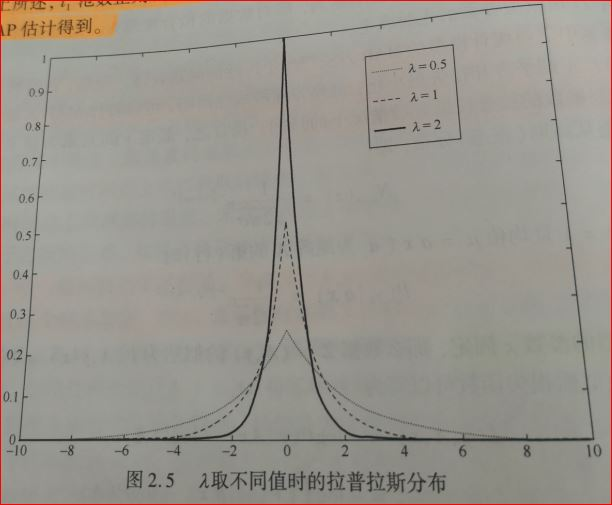
\includegraphics[width=0.7\linewidth]{Img/chap_srt01_problem/lap_lambda}
	\caption{$ \lambda $取不同值时的拉普拉斯分布}
	\label{fig:laplambda}
\end{figure}


当参数具有拉普拉斯先验时,正则函数可以写成
\begin{equation}\label{key}
\begin{split}
R(x,\lambda) &= -\log P(x|\lambda) = -\log \prod_i^{n}p(x_i|\lambda) \\
             &= \lambda\sum_i^n |x_i| +const
\end{split}
\end{equation}

其中$const=-\log\frac{\lambda}{2} $并不依赖于$ x $,因此可以从正则化损失最小化
问题中省略此项。从而产生如下为人熟悉的正则函数
\begin{equation*}\label{key}
R(x,\lambda) = \lambda\sum_i^n |x_i| = \Vert x\Vert_1
\end{equation*}


如上所述,$ \ell_1 $范数正则线性回归问题可以从参数具有拉普拉斯先验的线性观测模型中通过MAP估计得到。


\section{扩展$ LASSO $:其他损失函数与正则函数}












          %稀疏表达问题描述
%\chapter{理论结果:解的唯一性与不确定性}\label{chap:srt02:theory}

\section{引言}

\section{稀疏表示与字典学习}

\section{稀疏表示问题的求解}

\section{稀疏表示求解算法的理论分析}



\section{基于卷积神经网络的稀疏建模介绍}

           %稀疏表达理论问题
%
\part{稀疏表示:在图像处理中的应用}
%\chapter{图像锐化—专题研究}\label{chap:sra:sharpen}


本章我们将介绍稀疏域模型在图像锐化中的应用。


\section{问题描述}


\section{字典}

\section{数值计算上的考虑}


\section{实验结果与分析}             %图像锐化
%\chapter{字典的探索}\label{chap:sra:sharpen}


本章我们将介绍稀疏域模型在图像锐化中的应用。


\section{选择和学习的对比}



\section{字典学习算法}


\subsection{字典学习的核心问题}

\subsection{MOD算法}


\subsection{KSVD算法}



\section{结构化字典的训练}          %字典探索
%%%\input{Tex/Chap_SRC01_sparsePCA}        %图像压缩
%%%\input{Tex/Chap_SRC01_sparsePCA}        %图像去噪
%%%\input{Tex/Chap_SRC01_sparsePCA}    %图像超分辨率
\part{稀疏表示:\\在图像分类中的应用}
%%%\input{Tex/Chap_SRC01_sparsePCA}    %图像超分辨率

\part{附录:相关预备知识}
\chapter{抽象空间}\label{chap:introduction}

\section{引言}

\section{赋范空间}
设$X$是数域$K$上的向量空间($K=R$或$C$),若对每个$x\in X$指定一个实数$||x||$,称为x的范数,其满足以下范数公理。
\indent
\begin{description}
	\item[($N_1$)] 齐次性     \quad\qquad $||ax||=|a|\cdot||x||\quad a\in K$
	\item[($N_2$)] 三角不等式 \quad $||x+y|| \leq ||x|| + ||y||$
	\item[($N_3$)] 正定性     \quad\qquad $||x||\geq 0,\quad ||x||=0 \leftrightarrow  ||x||=0$
\end{description}
则称X为K上的赋范向量空间,简称赋范空间。

\noindent 注:
\begin{description}
	\item[1] 如K=R,称为实赋范空间,如K=C,则称为复赋范空间。
    \item[2] description
    \begin{description}
    	\item[a.] 称$|x| = \sqrt{\sum_i |x_i|^2}$称为Euclid范数,常用于解释赋范空间的模型。
    	\item[b.] 一般范数无具体计算公式,其本质在于范数公理,正是舍弃了特殊的表达式,才得到了具有高度抽象性的赋范空间理论。
    	\item[c.] 一旦将赋范空间理论应用于某个特定空间,就必须选择适当的范数公式。
    \end{description}
\end{description}


\noindent 
例:{\heiti 有界函数空间$B(\Omega)$}

设$\Omega$是任一非空集合,$B(\Omega)$是定义在$\Omega$上的有界实(复)函数之全体。其显然是一实(复)向量空间。
任给$\mu\in B(\Omega)$,令
$$||\mu||_0 =  \sup_{x\in\Omega} |\mu(x)|$$
\noindent 验证:
\begin{description}
	\item[$1^0$] 齐次性
	  $$||a\mu||_0 =  \sup_{x\in\Omega} |a\mu(x)|$$
	\item[$2^0$] 三角不等式
%	\begin{split}
		
%	\end{split}
	\item[$3^0$] 正定性
\end{description}
[说明]
\begin{enumerate}
	\item 自然数集$ N $上的有界函数就是有界数列。因此,有界数列空间$ B(N) $是一赋范空间,通常记做$ \ell^{\infty} $。
	
\end{enumerate}



设$ X $是一个给定的赋范空间,借用几何术语,赋予抽象概念以某种直观形象。
\begin{enumerate}
	\item [(1)] $ X $中的点成为点或向量,向量x可解释为从零元0到点x的有向线段。
	\item [(2)] $ \Vert x\Vert $称为$ x $的长度,当$\Vert x\Vert =1$ 时,称$ x $为单位向量。
	\item [(3)] 称 $ \Vert x-y\Vert $为点$ x $与点$ y $之间的距离,也记做$ d(x,y) $。
	\item [(4)] 
\end{enumerate}

\section{Banach空间}

\section{常用函数空间}

\section{内积空间与Hilbert空间}
                   %预备知识
%---------------------------------------------------------------------------%
% main content
%-
%-> Appendix
%-
\cleardoublepage%   
%\appendix% initialize the environment
%\chapter{中国科学院大学学位论文撰写要求}

学位论文是研究生科研工作成果的集中体现,是评判学位申请者学术水平、授予其学位的主要依据,是科研领域重要的文献资料。根据《科学技术报告、学位论文和学术论文的编写格式》(GB/T 7713-1987)、《学位论文编写规则》(GB/T 7713.1-2006)和《文后参考文献著录规则》(GB7714—87)等国家有关标准,结合中国科学院大学(以下简称“国科大”)的实际情况,特制订本规定。

\section{论文无附录者无需附录部分}

\section{测试公式编号} \label{sec:testmath}

\begin{equation} \label{eq:appedns}
    \begin{cases}
        \frac{\partial \rho}{\partial t} + \nabla\cdot(\rho\Vector{V}) = 0 \ \mathrm{times\ font\ test}\\
        \frac{\partial (\rho\Vector{V})}{\partial t} + \nabla\cdot(\rho\Vector{V}\Vector{V}) = \nabla\cdot\Tensor{\sigma} \ \text{times font test}\\
        \frac{\partial (\rho E)}{\partial t} + \nabla\cdot(\rho E\Vector{V}) = \nabla\cdot(k\nabla T) + \nabla\cdot(\Tensor{\sigma}\cdot\Vector{V})
    \end{cases}
\end{equation}
\begin{equation}
    \frac{\partial }{\partial t}\int\limits_{\Omega} u \, \mathrm{d}\Omega + \int\limits_{S} \unitVector{n}\cdot(u\Vector{V}) \, \mathrm{d}S = \dot{\phi}
\end{equation}

\section{测试生僻字}

霜蟾盥薇曜灵霜颸妙鬘虚霩淩澌菀枯菡萏泬寥窅冥毰毸濩落霅霅便嬛岧峣瀺灂姽婳愔嫕飒纚棽俪緸冤莩甲摛藻卮言倥侗椒觞期颐夜阑彬蔚倥偬澄廓簪缨陟遐迤逦缥缃鹣鲽憯懔闺闼璀错媕婀噌吰澒洞阛闠覼缕玓瓑逡巡諓諓琭琭瀌瀌踽踽叆叇氤氲瓠犀流眄蹀躞赟嬛茕頔璎珞螓首蘅皋惏悷缱绻昶皴皱颟顸愀然菡萏卑陬纯懿犇麤掱暒 墌墍墎墏墐墒墒墓墔墕墖墘墖墚墛坠墝增墠墡墢墣墤墥墦墧墨墩墪樽墬墭堕墯墰墱墲坟墴墵垯墷墸墹墺墙墼墽垦墿壀壁壂壃壄壅壆坛壈壉壊垱壌壍埙壏壐壑壒压壔壕壖壗垒圹垆壛壜壝垄壠壡坜壣壤壥壦壧壨坝塆圭嫶嫷嫸嫹嫺娴嫼嫽嫾婳妫嬁嬂嬃嬄嬅嬆嬇娆嬉嬊娇嬍嬎嬏嬐嬑嬒嬓嬔嬕嬖嬗嬘嫱嬚嬛嬜嬞嬟嬠嫒嬢嬣嬥嬦嬧嬨嬩嫔嬫嬬奶嬬嬮嬯婴嬱嬲嬳嬴嬵嬶嬷婶嬹嬺嬻嬼嬽嬾嬿孀孁孂娘孄孅孆孇孆孈孉孊娈孋孊孍孎孏嫫婿媚嵭嵮嵯嵰嵱嵲嵳嵴嵵嵶嵷嵸嵹嵺嵻嵼嵽嵾嵿嶀嵝嶂嶃崭嶅嶆岖嶈嶉嶊嶋嶌嶍嶎嶏嶐嶑嶒嶓嵚嶕嶖嶘嶙嶚嶛嶜嶝嶞嶟峤嶡峣嶣嶤嶥嶦峄峃嶩嶪嶫嶬嶭崄嶯嶰嶱嶲嶳岙嶵嶶嶷嵘嶹岭嶻屿岳帋巀巁巂巃巄巅巆巇巈巉巊岿巌巍巎巏巐巑峦巓巅巕岩巗巘巙巚帠帡帢帣帤帨帩帪帬帯帰帱帲帴帵帷帹帺帻帼帽帾帿幁幂帏幄幅幆幇幈幉幊幋幌幍幎幏幐幑幒幓幖幙幚幛幜幝幞帜幠幡幢幤幥幦幧幨幩幪幭幮幯幰幱庍庎庑庖庘庛庝庠庡庢庣庤庥庨庩庪庬庮庯庰庱庲庳庴庵庹庺庻庼庽庿廀厕廃厩廅廆廇廋廌廍庼廏廐廑廒廔廕廖廗廘廙廛廜廞庑廤廥廦廧廨廭廮廯廰痈廲廵廸廹廻廼廽廿弁弅弆弇弉弖弙弚弜弝弞弡弢弣弤弨弩弪弫弬弭弮弰弲弪弴弶弸弻弼弽弿彖彗彘彚彛彜彝彞彟彴彵彶彷彸役彺彻彽彾佛徂徃徆徇徉后徍徎徏径徒従徔徕徖徙徚徛徜徝从徟徕御徢徣徤徥徦徧徨复循徫旁徭微徯徰徱徲徳徴徵徶德徸彻徺忁忂惔愔忇忈忉忔忕忖忚忛応忝忞忟忪挣挦挧挨挩挪挫挬挭挮挰掇授掉掊掋掍掎掐掑排掓掔掕挜掚挂掜掝掞掟掠采探掣掤掦措掫掬掭掮掯掰掱掲掳掴掵掶掸掹掺掻掼掽掾掿拣揁揂揃揅揄揆揇揈揉揊揋揌揍揎揑揓揔揕揖揗揘揙揤揥揦揧揨揫捂揰揱揲揳援揵揶揷揸揻揼揾揿搀搁搂搃搄搅搇搈搉搊搋搌搎搏搐搑搒摓摔摕摖摗摙摚摛掼摝摞摠摡斫斩斮斱斲斳斴斵斶斸旪旫旮旯晒晓晔晕晖晗晘晙晛晜晞晟晠晡晰晣晤晥晦晧晪晫晬晭晰晱晲晳晴晵晷晸晹晻晼晽晾晿暀暁暂暃暄暅暆暇晕晖暊暋暌暍暎暏暐暑暒暓暔暕暖暗旸暙暚暛暜暝暞暟暠暡暣暤暥暦暧暨暩暪暬暭暮暯暰昵暲暳暴暵暶暷暸暹暺暻暼暽暾暿曀曁曂曃晔曅曈曊曋曌曍曎曏曐曑曒曓曔曕曗曘曙曚曛曜曝曞曟旷曡曢曣曤曥曦曧昽曩曪曫晒曭曮曯椗椘椙椚椛検椝椞椟椠椡椢椣椤椥椦椧椨椩椪椫椬椭椮椯椰椱椲椳椴椵椶椷椸椹椺椻椼椽椾椿楀楁楂楃楅楆楇楈楉杨楋楌楍榴榵榶榷榸榹榺榻榼榽榾桤槀槁槂盘槄槅槆槇槈槉槊构槌枪槎槏槐槑槒杠槔槕槖槗滙滛滜滝滞滟滠滢滣滦滧滪滫沪滭滮滰滱渗滳滵滶滹滺浐滼滽漀漃漄漅漈漉溇漋漌漍漎漐漑澙熹漗漘漙沤漛漜漝漞漟漡漤漥漦漧漨漪渍漭漮漯漰漱漳漴溆漶漷漹漺漻漼漽漾浆潀颍潂潃潄潅潆潇潈潉潊潋潌潍潎潏潐潒潓洁潕潖潗潘沩潚潜潝潞潟潠潡潢潣润潥潦潧潨潩潪潫潬潭浔溃潱潲潳潴潵潶滗潸潹潺潻潼潽潾涠澁澄澃澅浇涝澈澉澊澋澌澍澎澏湃澐澑澒澓澔澕澖涧澘澙澚澛澜澝澞澟渑澢澣泽浍澯澰淀澲澳澴澵澶澷澸潇潆瀡瀢瀣瀤瀥潴泷濑瀩瀪瀫瀬瀭瀮瀯弥瀱潋瀳瀴瀵瀶瀷瀸瀹瀺瀻瀼瀽澜瀿灀灁瀺灂沣滠灅灆灇灈灉灊灋灌灍灎灏灐洒灒灓漓灖灗滩灙灚灛灜灏灞灟灠灡灢湾滦灥灦灧灨灪燝燞燠燡燢燣燤燥灿燧燨燩燪燫燮燯燰燱燲燳烩燵燵燸燹燺薰燽焘燿爀爁爂爃爄爅爇爈爉爊爋爌烁爎爏爑爒爓爔爕爖爗爘爙爚烂爜爝爞爟爠爡爢爣爤爥爦爧爨爩猽猾獀犸獂獆獇獈獉獊獋獌獍獏獐獑獒獓獔獕獖獗獘獙獚獛獜獝獞獟獠獡獢獣獤獥獦獧獩狯猃獬獭狝獯狞獱獳獴獶獹獽獾獿猡玁玂玃。
% appendix content
%-
%-> Backmatter: bibliography, glossary, index
%-
%\backmatter% initialize the environment
\intotoc{\bibname} % add link to contents table and bookmark
%\bibliography{Biblio/ref}% bibliography
%\chapter{作者简历及攻读学位期间发表的学术论文与研究成果}

\textbf{本科生无需此部分}。

\section*{作者简历}

\subsection*{casthesis作者}

吴凌云,福建省屏南县人,中国科学院数学与系统科学研究院博士研究生。

\subsection*{ucasthesis作者}

莫晃锐,湖南省湘潭县人,中国科学院力学研究所硕士研究生。

\section*{已发表(或正式接受)的学术论文:}

[1] ucasthesis: A LaTeX Thesis Template for the University of Chinese Academy of Sciences, 2014.

\section*{申请或已获得的专利:}

(无专利时此项不必列出)

\section*{参加的研究项目及获奖情况:}

可以随意添加新的条目或是结构。

\chapter[致谢]{致\quad 谢}\chaptermark{致\quad 谢}% syntax: \chapter[目录]{标题}\chaptermark{页眉}
\thispagestyle{noheaderstyle}% 如果需要移除当前页的页眉
%\pagestyle{noheaderstyle}% 如果需要移除整章的页眉

感激casthesis作者吴凌云学长,gbt7714-bibtex-style
开发者zepinglee,和ctex众多开发者们。若没有他们的辛勤付出和非凡工作,\LaTeX{}菜鸟的我是无法完成此国科大学位论文\LaTeX{}模板ucasthesis的。在\LaTeX{}中的一点一滴的成长源于开源社区的众多优秀资料和教程,在此对所有\LaTeX{}社区的贡献者表示感谢!

ucasthesis国科大学位论文\LaTeX{}模板的最终成型离不开以霍明虹老师和丁云云老师为代表的国科大学位办公室老师们制定的官方指导文件和众多ucasthesis用户的热心测试和耐心反馈,在此对他们的认真付出表示感谢。特别对国科大的赵永明同学的众多有效反馈意见和建议表示感谢,对国科大本科部的陆晴老师和本科部学位办的丁云云老师的细致审核和建议表示感谢。谢谢大家的共同努力和支持,让ucasthesis为国科大学子使用\LaTeX{}撰写学位论文提供便利和高效这一目标成为可能。

\cleardoublepage[plain]% 让文档总是结束于偶数页,可根据需要设定页眉页脚样式,如 [noheaderstyle]

% other information
\end{document}
%---------------------------------------------------------------------------%

